%%%%%%%%%%%%%%%%%%%%%%%%%%%%%%%%%%%%%%%%%
% Tutorial
% LaTeX Template
% Version 1.0 (09/27/17)
%
% Author:
% Ben Roose (ben.roose@wichita.edu)
%
% Original template author:
% Adam Glesser (adamglesser@gmail.com)
% www.LaTeXTemplates.com
%
% License:
% CC BY-NC-SA 3.0 (http://creativecommons.org/licenses/by-nc-sa/3.0/)
%
%%%%%%%%%%%%%%%%%%%%%%%%%%%%%%%%%%%%%%%%%

\documentclass[12pt]{article}

\usepackage{graphicx} % Allow import of images
\usepackage{subcaption} % Required for side-by-side sub figures
\graphicspath{ {images/} } % Relative path to images directory
\usepackage[margin=1in]{geometry} % Required to make the margins smaller to fit more content on each page
\usepackage[linkcolor=blue]{hyperref} % Required to create hyperlinks to questions from elsewhere in the document
\hypersetup{pdfborder={0 0 0}, colorlinks=true, urlcolor=blue} % Specify a color for hyperlinks
\usepackage{todonotes} % Required for the boxes that questions appear in
\usepackage{tocloft} % Required to give customize the table of contents to display questions
\usepackage{microtype} % Slightly tweak font spacing for aesthetics
\usepackage{palatino} % Use the Palatino font
\usepackage{listings} % Required for Bash command lines
\usepackage[T1]{fontenc} % Properly formats tildes (~) for command-line use

\setlength\parindent{0pt} % Removes all indentation from paragraphs

% Create and define the list of questions
\newlistof{questions}{faq}{\large FAQ for SSH access into cslab Linux environment}
% This creates a new table of contents-like environment that will output a file with extension .faq
\setlength\cftbeforefaqtitleskip{3em} % Adjusts the vertical space between the title and subtitle
\setlength\cftafterfaqtitleskip{1em} % Adjusts the vertical space between the subtitle and the first question
\setlength\cftparskip{.3em} % Adjusts the vertical space between questions in the list of questions

% Create the command used for questions
\newcommand{\question}[1] % This is what you will use to create a new question
{
\refstepcounter{questions} % Increases the questions counter, this can be referenced anywhere with \thequestions
%\hfill
\goodbreak
\par\noindent % Creates a new unindented paragraph
\phantomsection % Needed for hyperref compatibility with the \addcontensline command
\addcontentsline{faq}{questions}{#1} % Adds the question to the list of questions
\todo[inline, color=green!40]{\textbf{#1}} % Uses the todonotes package to create a fancy box to put the question
%\vspace{0.5em} % White space after the question before the start of the answer
}

% Uncomment the line below to get rid of the trailing dots in the table of contents
%\renewcommand{\cftdot}{}

% Uncomment the two lines below to get rid of the numbers in the table of contents
%\let\Contentsline\contentsline
%\renewcommand\contentsline[3]{\Contentsline{#1}{#2}{}}

\begin{document}

%----------------------------------------------------------------------------------------
%	TITLE AND LIST OF QUESTIONS
%----------------------------------------------------------------------------------------

\begin{center}
\Huge{\bf \emph{EECS Tutorial: cslab Linux Environment SSH Access}} % Main title
\end{center}

\listofquestions % This prints the subtitle and a list of all of your questions
\bigskip % Create a gap between list and first question
\href{https://github.com/benroose/tutorials/blob/master/cslab_tutorials/eecs_tutorial_cslab_web_access.pdf}{For web-browser access into cslab see eecs\_tutorial\_cslab\_web\_access}

\newpage % Comment this if you would like your questions and answers to start immediately after table of questions

%----------------------------------------------------------------------------------------
%	QUESTIONS AND ANSWERS
%----------------------------------------------------------------------------------------
\begin{flushleft}

\question{General Information regarding accessing cslab Linux environment using SSH}\label{ssh_client_linux}
\begin{itemize}
  \item \textbf{Only connect to the cslab environment with an SSH client if you have previous experience in using SSH and the Linux command-line. If you are new to Linux, please use the cslab web-browser interface at \href{https://cslab-gateway.cs.wichita.edu/}{cslab-gateway.cs.wichita.edu}.}
  \item SSH uses network port 22. When accessing cslab via SSH on WSU campus, ensure you are connected wirelessly to \textit{WSU Secure} or using an Ethernet connection. \textit{WSU Guest} prohibits port 22 connections so SSH conections will not work.
  \item You can only access cslab using SSH public key authentication. You cannot access cslab over SSH using your myWSU password.
  \item cslab-nodes are located inside a private network and only accessible via the \verb|cslab-bastion| jumphost. Any external connection into the cslab environment must proxy through \verb|cslab-bastion.cs.wichita.edu|.
  \item \verb|cslab-sftp.cs.wichita.edu| can be used for secure file transfer with command-line tools, such as \textit{PSFTP/SFTP}, or graphical tools, such as \textit{Filezilla}.
  \item This tutorial will help you configure your SSH and SFTP clients for access into cslab using SSH public key authentication via the \verb|cslab-bastion| jumphost.
  \item \textbf{ONLY USE CSLAB-BASTION AS A PROXY/JUMPHOST AND CSLAB-SFTP AS AN SCP/SFTP SERVER. DO NOT DIRECTLY SSH INTO CSLAB-BASTION OR CSLAB-SFTP FOR ANY OTHER TASKS!}
\end{itemize}

\begin{figure}[bh!]
  \centering
  %% \begin{subfigure}{.5\textwidth}
  \centering
  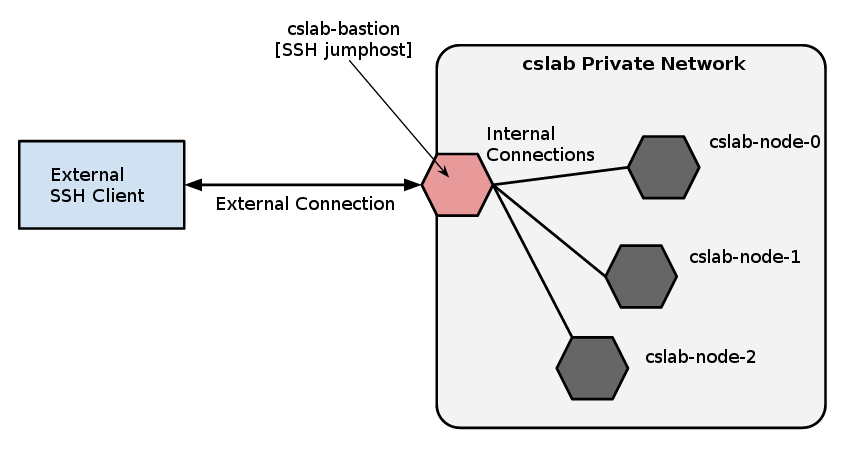
\includegraphics[width=.9\linewidth]{cslab_ssh_network}
\caption{Logical diagram of cslab network}
  \label{fig:pageant}
%% \end{subfigure}%
\end{figure}


%------------------------------------------------
\newpage
\question{How do I access cslab Linux environment via \textit{PuTTY} on Microsoft Windows?}\label{ssh_client_windows}
  
\subsection*{Configuring the \textit{PuTTY} SSH client for cslab access:}
\begin{enumerate}
  \item Download the full \textit{PuTTY} package from \href{https://www.chiark.greenend.org.uk/~sgtatham/putty/latest.html}{Simon Tatham's official download page} and install all \textit{PuTTY} utilities on your local Windows computer. You cannot connect to cslab with just the \textit{PuTTY} client.
  \item Run the \textit{PuTTY Key Generator}, which is listed in your start menu as \textit{PuTTYgen}.
  \item In the \textit{PuTTY Key Generator} window, generate a new RSA key with 4096 bits. You may need to change the settings at bottom of window before clicking \textbf{Generate}.
  \item Follow the prompts to create randomness and generate your \textit{PuTTY} key.
  \item Once your key has been generated, change the following fields:
    \begin{itemize}
    \item Key comment: \verb|your_mywsu_id@your_local_computer_name|
    \item Key passphrase: \verb|choose_passphrase_you_will_remember|
    \item Confirm passphrase: \verb|same_passphrase_as_above|
    \end{itemize}
    \textbf{It is highly recommended to use a passphrase for your new key to keep your Linux user account secure.}
  \item Select all the text displayed within the box titled \textit{Public key for pasting into OpenSSH authorized\_keys file}, starting with \texttt{ssh-rsa} and ending with name of your computer.
  \item Copy the selected text either by right-clicking within the same box and selecting [copy] or by pressing the key combination \textbf{Ctrl+C}.
  \item Open a web-browser application and follow the \href{https://github.com/benroose/tutorials/blob/master/cslab_tutorials/eecs_tutorial_cslab_web_access.pdf}{eecs\_tutorial\_cslab\_web\_access} document to access \href{https://cslab-gateway.cs.wichita.edu/}{cslab-gateway.cs.wichita.edu}
  \item Once logged into \textit{guacamole}, open a \textbf{cslab\_SSH\_CLI\_terminal} connection.
  \item Within the cslab SSH terminal session in your browser, open the \textit{Guacamole} menu sidebar by pressing the key combination \textbf{Ctrl+Alt+Shift}.
  \item Paste the copied text to the remote \textit{Guacamole} \textbf{Clipboard} field using your preferred method, i.e. \textbf{Ctrl+V}.
  \item Close the \textit{Guacamole} menu sidebar by pressing the key combination \textbf{Ctrl+Alt+Shift}.
  \item Within the cslab SSH terminal session, open your \verb|authorized_keys| file by typing \break
    \verb|nano ~/.ssh/authorized_keys|
  \item Paste your locally copied \textit{PuTTY} SSH public key into the terminal session by right-clicking on the browser window with your mouse or by pressing the key combination \textbf{Ctrl+Shift+V}.
  \item Ensure you have a blank line at end of the text file by pressing \textbf{Enter} if required.
  \item Quit \textit{nano} by pressing \textbf{CTRL+X} and follow the prompts at the bottom of the screen to ensure you save the \verb|authorized_keys| file.
  \item Ensure correct permissions are set on the \verb|authorized_keys| file by typing \break
    \verb|chmod 600 ~/.ssh/authorized_keys|
  \item NOTE: If you wish to set up more than one local computer with different SSH keys for accessing cslab, then you can append additional SSH public keys in your cslab user \verb|authorized_keys| file. Make sure to remove no longer used SSH public keys from this file.
  \item Once you are done with the above steps, make sure to properly disconnect and log out of the cslab \textit{guacamole} web-interface.
  \item Back in the \textit{PuTTY Key Generator} window, click \textbf{Save private key}.
  \item In the \textit{Save private key} window, browse to a local directory where you wish to securely store your new \textit{PuTTY} SSH key and in the \textbf{File name} field enter the name \verb|cslab_rsa|. Clicking on \textbf{Save} will store your \verb|cslab_rsa.ppk| key file to your local computer. \textbf{Keep this file safe and private!}
  \item OPTIONAL: If you wish to also store your SSH public key as a simple text file for future reference, then click \textbf{Save public key}, browse to the same directory, and in the \textbf{File name} field enter the name \verb|cslab_rsa_public_key.txt|
  \item Once you are done with the above steps, exit/close the \textit{PuTTY Key Generator} program.
  \item Download the \href{https://raw.githubusercontent.com/benroose/tutorials/master/cslab_tutorials/cslab_ssh_client_config_files/cslab_putty_ssh_client_full_configuration.reg}{cslab\_putty\_ssh\_client\_full\_configuration.reg} registry file from \href{https://github.com/benroose/tutorials/tree/master/cslab_tutorials/}{Ben Roose's GitHub tutorials repository}. You may need to right-click on the web-page in your browser and select \textbf{Save as} or \textbf{Save page as}.
  \item Double-click on the downloaded file in your file explorer, and click \textbf{Yes} when asked if you wish to add this new information to your Windows registry. You will not be able to continue configuration of PuTTY until this file has been added into your Windows registry.
  \item Run the \textit{PuTTY} program and you should now see two new \textbf{Saved Sessions} entries in your \textit{PuTTY} Configuration Window listed as \textit{cslab access} and \textit{cslab last node accessed}.
  \item Click on \textit{cslab access} and click on \textbf{Load}. DO NOT click \textbf{Open}.
  \item Click on the \textit{Connection--Data} Category tab on the left of the window and enter your myWSU ID in the \textbf{Auto-login username} field.
  \item Click on the \textit{Connection--Proxy} Category tab on the left of the window and enter your myWSU ID in the \textbf{Username} field.
  \item Click on the \textit{Session} Category tab on the left of the window and click on \textbf{Save}. DO NOT click \textbf{Open}.
  \item Perform the last 4 steps again for the \textit{cslab last node accessed} entry.
  \item Once you are done with the above steps, exit/close the \textit{PuTTY} program.
  \item Congratulations! You have now configured your local Windows computer to directly access cslab with \textit{PuTTY}. However, you will need to add your new SSH key to the \textit{Pageant (PuTTY Authentication agent)} prior to logging into cslab. Running \textit{Pageant} and adding your SSH key will be explained in the next section.
\end{enumerate}

\begin{figure}[bh!]
\centering
\begin{subfigure}{.5\textwidth}
  \centering
  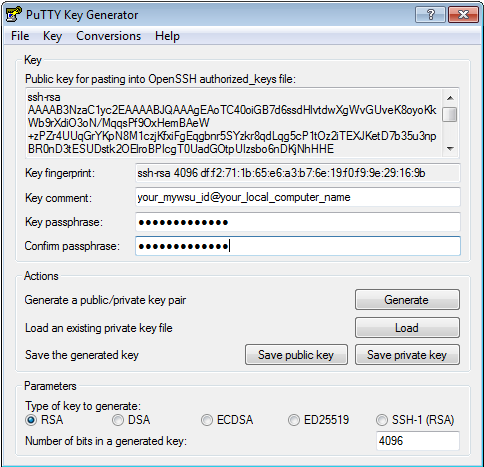
\includegraphics[width=.9\linewidth]{puttygen_key_gen_fields}
  %% \caption{A subfigure}
  \label{fig:sub1}
\end{subfigure}%
\begin{subfigure}{.5\textwidth}
  \centering
  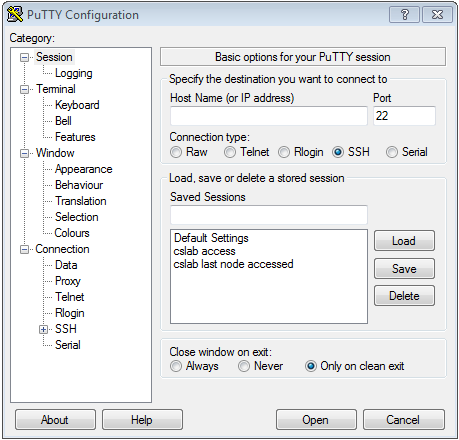
\includegraphics[width=.9\linewidth]{putty_cslab_session_tab}
  %% \caption{A subfigure}
  \label{fig:sub2}
\end{subfigure}
\begin{subfigure}{.5\textwidth}
  \centering
  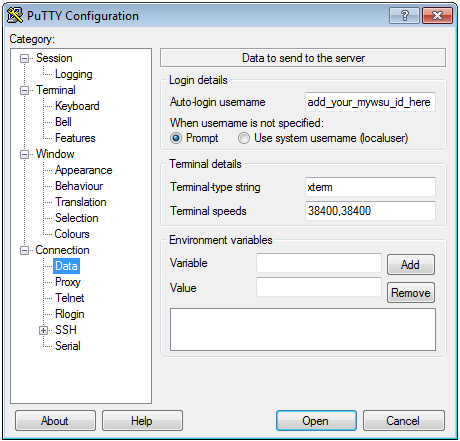
\includegraphics[width=.9\linewidth]{putty_cslab_data_tab}
  %% \caption{A subfigure}
  \label{fig:sub3}
\end{subfigure}%
\begin{subfigure}{.5\textwidth}
  \centering
  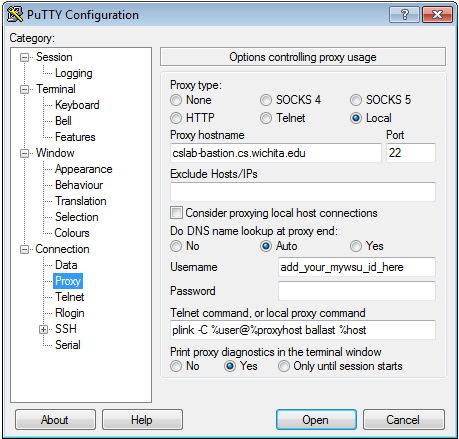
\includegraphics[width=.9\linewidth]{putty_cslab_proxy_tab}
  %% \caption{A subfigure}
  \label{fig:sub4}
\end{subfigure}%
\caption{\textit{PuTTY} screenshots for cslab configuration}
\label{fig:putty_config}
\end{figure}

\newpage
\subsection*{Logging into cslab using the \textit{Pageant} agent:}
\begin{enumerate}
  \item Run the \textit{Pageant (PuTTY Authentication agent)}, listed in your start menu as \textit{Pageant}.
  \item On the far right of your Windows taskbar, you should see a new notification icon for the running \textit{Pageant} program.
  \item Right-click on the \textit{Pageant} notification icon and select the menu option \textbf{Add key}.
  \item In the \textit{Select private Key File} window, browse to the local directory with your stored \verb|cslab_rsa.ppk| file. Select the \texttt{cslab\_rsa} key file and click on \textbf{Open}.
  \item When prompted, enter the previously defined passphrase for your key.
  \item OPTIONAL: if you wish to see the SSH keys already added into \textit{Pageant}, right-click on the \textit{Pageant} notification icon and select the menu option \textbf{View keys}.
  \item Right-click on the \textit{Pageant} notification icon and, under the \textbf{Saved Sessions} sub-menu, select \textbf{cslab remote access}.
  \item If everything is correctly configured, a \textit{PuTTY} terminal emulator window will open and automatically log you into an available cslab node! You should be presented with the shell prompt: 
    \verb|your_mywsu_id@cslab-node-#:~$|
  %%   You should be presented with a standard shell prompt within the node: \break
  %% \verb|your_mywsu_id@cslab-node-#:~$|
  \item Each time you shutdown or reboot your computer, you will need to manually run \textit{Pageant} and then add your SSH key before you can connect to the cslab environment.
  \item OPTIONAL: You can have \textit{Pageant} run automatically at startup by copying the \textit{Pageant} Start menu shortcut file into your Windows \textbf{Startup} directory.
  \item OPTIONAL: To have your cslab SSH key automatically added into \textit{Pageant} when it runs, open the \textbf{Properties} box for the \textit{Pageant} Start menu shortcut (or the previously created \textbf{Startup} shortcut). In the \textbf{Target} field append the full filepath of your \verb|cslab_rsa.ppk| key file to the end of the \verb|pageant.exe| line, i.e.
\end{enumerate}
  \begin{verbatim}
"C:\Program Files\PuTTY\pageant.exe" "C:\Users\localuser\cslab_rsa.ppk"
  \end{verbatim}

\begin{figure}[bh!]
  \centering
  %% \begin{subfigure}{.5\textwidth}
  \centering
  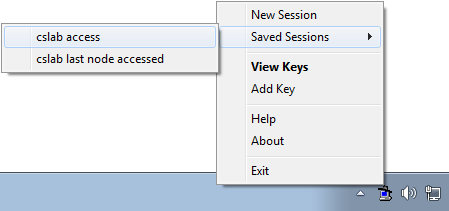
\includegraphics[width=.5\linewidth]{pageant_taskbar_menu}
\caption{\textit{Pageant} taskbar menu for cslab access}
  \label{fig:pageant}
%% \end{subfigure}%
\end{figure}

%------------------------------------------------
\newpage
\subsection*{Logging into your last used cslab-node-\# using the \textit{PuTTY} client:}
\begin{itemize}
  \item When connecting to the cslab Linux environment using an SSH client, the \textit{ballast} load-balancer will redirect you to one of the available and least used cslab-nodes at time of connection. Since load-balancing is calculated by \textit{ballast} on a one minute cycle, you may not be redirected to the same cslab-node each time you connect.

  \item \textbf{Use the \textit{cslab last node accessed} saved session to connect to the last used cslab-node only when you need access into a previously running SSH session. For normal use the best option is to connect using the \textit{cslab access} saved session and let the \textit{ballast} load-balancer automatically connect to an available node.}
\end{itemize}

\subsection*{Running graphical (GUI) applications using the \textit{PuTTY} client:}
\begin{enumerate}
  \item SSH allows for graphical applications to run on a local computer from the remote cslab Linux environment using X11 forwarding.
  \item You will need to install the Xming software before using X11 forwarding with \textit{PuTTY}. Download the \href{http://sourceforge.net/project/downloading.php?group_id=156984&filename=Xming-6-9-0-31-setup.exe}{Xming X Server for Windows} and install the software package.
  \item Run the \textit{PuTTY} program, click on \textbf{cslab access} in Saved Sessions, and click on \textbf{Load}.
  \item Click on the \textit{Connection--SSH--X11} Category tab on the left of the window.
  \item Turn on the \textbf{Enable X11 Forwarding} check box and ensure the \textbf{X display location} contains \texttt{localhost:0.0}. If you change the display location within \textit{Xming Launch} settings, then also change the \textbf{X display location} in \textit{PuTTY} to ensure consistency.
  \item Click on the \textit{Session} Category tab on the left of the window. Save this change as a different \textbf{Saved Session} by entering a new name for the session, such as \texttt{cslab with graphical access}, and click on \textbf{Save}.
  \item Once you are done with the above steps, exit/close the \textit{PuTTY} program.
  \item To use cslab with X11 forwarding, first run \textit{Xming} in the background and then select your new \textbf{Saved Session} from the \textit{Pageant} notification menu.
  \item Once a connection into cslab has been established, you can type the name of a GUI application you wish to run, such as \verb|geany &|
\end{enumerate} 

%% \begin{figure}[bh!]
%%   \centering
%%   %% \begin{subfigure}{.5\textwidth}
%%   \centering
%%   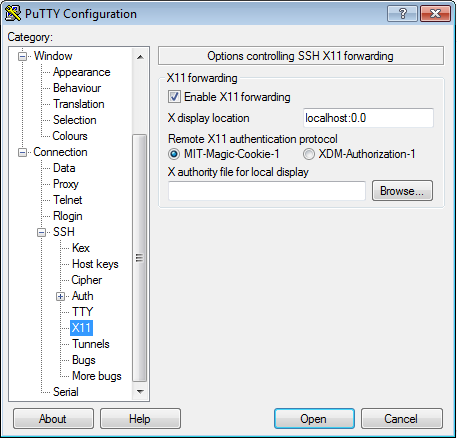
\includegraphics[width=.5\linewidth]{cslab_x11_tab}
%% %% \caption{\textit{PuTTY} Enable X11 Forwarding}
%%   \label{fig:x11_forwarding}
%% %% \end{subfigure}%
%% \end{figure}

%------------------------------------------------
\newpage
\question{How do I copy files from/to cslab Linux environment via SSH on Windows?}\label{sftp_windows}

\subsection*{Copying files remotely using \textit{PuTTY} command-line tools:}
\begin{itemize}
  \item Ensure you have first followed the directions in the previous section to configure your \textit{PuTTY} client and \textit{pagant} is running with your SSH private key added.
  \item Open a Windows command prompt window.
  \item To copy a file from your local computer to your user home directory on cslab using \textit{PuTTY Secure Copy (PSCP)}, type
    \verb|pscp local_file mywsu_id@cslab-sftp.cs.wichita.edu:remote_dir|
\item To copy a file from your user home directory on cslab to a local directory on your local computer using \textit{PuTTY Secure Copy (PSCP)}, type
  \verb|pscp mywsu_id@cslab-sftp.cs.wichita.edu:remote_file local_dir|
    
  \item To use \textit{PuTTY SSH File Transfer Protocol (PSFTP)} interactive command-line tool, type \break
  \verb|psftp mywsu_id@cslab-sftp.cs.wichita.edu|
  \item To see a list of available interactive commands once in \verb|psftp>|, type \verb|help|
  \item For further information on \verb|pscp| and \verb|psftp|, see the online \textit{PuTTY} documentation for \href{https://the.earth.li/~sgtatham/putty/0.60/htmldoc/Chapter5.html}{Chapter 5} and \href{https://the.earth.li/~sgtatham/putty/0.60/htmldoc/Chapter6.html}{Chapter 6} respectively.
\end{itemize}

\subsection*{Copying files remotely using \textit{SFTP} with the \textit{FileZilla} graphical client:}
\begin{enumerate}
  \item Ensure you have first followed the directions in the previous section to configure your \textit{PuTTY} client.
  \item Download \texttt{FileZilla} software from the \href{https://filezilla-project.org/download.php}{FileZilla download page} and install the SFTP client on your local Windows computer.
  \item Run the \textit{FileZilla} graphical client program.
  \item In the \textit{FileZilla} window, open the \textbf{Site Manager} via the \textbf{File} menu, by clicking on the upper-left icon, or by pressing \textbf{CTRL+S}.
  \item In \textit{Site Manager} window, click \textbf{New Site} and type in a site name, i.e. \verb|cslab-sftp|
  \item In \textit{Site Manager} window, change the following fields:
  \begin{itemize}
    \item Host: \verb|cslab-sftp.cs.wichita.edu|
    \item Protocol: \verb|[SFTP - SSH File Transfer Protocol]|
    \item Logon Type: \verb|[Key file]|
    \item User: \verb|your_mywsu_id|
  \end{itemize}
  \item \textit{FileZilla} can use \textit{PuTTY} SSH keys. To the right of the Key file field click \textbf{Browse}.
  \item In the \textit{Choose a key file} window, browse to the local directory with your stored \verb|cslab_rsa.ppk| file. Select the \texttt{cslab\_rsa} key file and click on \textbf{Open}.
  \item Click \textbf{Connect} and enter the passphrase/password to unlock your \textit{PuTTY} private key when prompted.
  \item If you have set up \textit{FileZilla} correctly, it will automatically connect to \verb|cslab-sftp| and display your home directory on cslab in the right pane.
  \item Drag-and-drop files to transfer them between your local computer and the remote cslab environment.
  \item If you wish to hide ``hidden'' files which start with a period, then select \textbf{Directory Listing Filters} under the \textbf{View} menu, enable \textit{Configuration files} on the Remote filter, and click \textbf{OK} or \textbf{Apply}.
  \item For further information on how to use \textit{FileZilla}, see the \href{https://wiki.filezilla-project.org/Documentation}{FileZilla documentation page}.
\end{enumerate}

\begin{figure}[th!]
  \centering
  %% \begin{subfigure}{.5\textwidth}
  \centering
  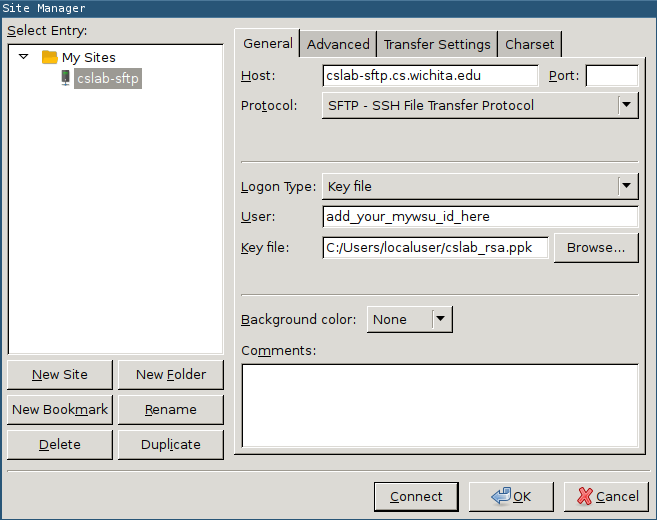
\includegraphics[width=.6\linewidth]{filezilla_cslab_site_manager_windows}
\caption{\textit{FileZilla} Site Manager settings for cslab-sftp}
  \label{fig:pageant}
%% \end{subfigure}%
\end{figure}

%------------------------------------------------
\newpage
\question{Why is \textit{PuTTY} or \textit{FileZilla} asking to confirm the authenticity of cslab host keys?}\label{host_keys_windows}

\subsection*{Automatically adding cslab host keys to your registry for \textit{PuTTY}:}
\begin{itemize}
  \item SSH host keys are essential to securing an SSH connection into a remote server. If you see an incorrect host key, then it may mean a cyber-attacker has attempted to compromise the remote server.
  \item The \href{https://raw.githubusercontent.com/benroose/tutorials/master/cslab_tutorials/cslab_ssh_client_config_files/cslab_putty_ssh_client_full_configuration.reg}{cslab\_putty\_ssh\_client\_full\_configuration.reg} registry file will automatically add the cslab host keys into your Windows registry during your initial configuration and set up of \textit{PuTTY}. However, if your configuration loses its cached host keys for any reason, then it may ask you to reconfirm the authenticity of cslab hosts when you try to open an SSH connection.
  \item You can download the \href{https://raw.githubusercontent.com/benroose/tutorials/master/cslab_tutorials/cslab_ssh_client_config_files/cslab_putty_ssh_client_host_keys_only.reg}{cslab\_putty\_ssh\_host\_keys\_only.reg} registry file and re-add just the cslab host keys into your Windows registry.

\end{itemize}

%% \newpage
\subsection*{Manually adding the cslab host keys into \textit{PuTTY} or \textit{FileZilla}:}
\begin{itemize}
  \item You can manually add SSH host keys to your \textit{PuTTY} and \textit{FileZilla} configurations. When adding new host keys you should always ensure the host key fingerprint is correct. \verb|cslab|, \verb|cslab-bastion|, and \verb|cslab-sftp| host key fingerprints must match one of the following SHA256 or MD5 hashes before you add or accept the host key:
\begin{verbatim}
ECDSA key fingerprint is
SHA256:X6dBKj4sqYYPWol6MXSQvGhpIQ6qBxh7mBQhnSw8n64
MD5:d8:ba:c6:1c:86:fa:7f:f6:92:4f:c1:02:30:ce:ab:99

ED25519 key fingerprint is
SHA256:zzozIV7cP1T9C77PLRaevzdzCu21k44lbjd8jaJKS8Q
MD5:6d:3d:8e:3a:db:f6:de:33:af:77:01:40:f3:71:1d:14

RSA key fingerprint is
SHA256:0CUyGZAYMdOd8vTOK3AtM2XTX3lMaGA2NP73rR7s6Ns
MD5:75:5a:16:53:1a:7c:c2:4b:99:66:2d:e3:1e:76:f9:c9

DSA key fingerprint is
SHA256:7zW122xr+aoBb5yiRI96nvdx8Ml07qLKHYwG2Wu6jIM
MD5:27:59:53:18:5a:67:71:f6:32:f1:e1:15:e9:e5:fe:b1
\end{verbatim}

\end{itemize}

%------------------------------------------------
\newpage
\question{How do I access cslab Linux environment via \textit{OpenSSH} on Linux or Mac?}\label{ssh_client_linux}

\subsection*{Configuring the \textit{OpenSSH} client for cslab access:}
\begin{enumerate}
  \item Many of the following commands need to be typed into a local command-line terminal, so open a command-line terminal emulator window first.
  \item Install the \texttt{openssh-client} software package using your specific distribution's package management tools if not already installed.
  \item Download the \href{https://raw.githubusercontent.com/benroose/tutorials/master/cslab_tutorials/cslab_ssh_client_config_files/cslab_openssh_client_config}{cslab\_openssh\_client\_config} file from \href{https://github.com/benroose/tutorials/tree/master/cslab_tutorials/}{Ben Roose's GitHub tutorials repository}. You may need to right-click on the web-page in your browser and select \textbf{Save as} or \textbf{Save page as}, or you can download this file directly using \verb|wget|
  \item The downloaded cslab configuration can be added into your SSH client config while substituting your own myWSU ID into it by changing into the directory where you downloaded the \verb|cslab_openssh_client_config| file and typing
\begin{verbatim}
sed "s/mywsu_placeholder/ENTER_YOUR_OWN_MYWSU_ID_HERE/g" \
 cslab_openssh_client_config >> ~/.ssh/config
\end{verbatim}
  \item Alternatively, you can manually copy the following host entries into your local \verb|~/.ssh/config| file:
\end{enumerate}

\begin{verbatim}
Host cslab cslab-last cslab.cs.wichita.edu cslab-last.cs.wichita.edu
  ProxyCommand ssh your_mywsu_id@cslab-bastion.cs.wichita.edu ballast %h
  User your_mywsu_id
  IdentityFile $HOME/.ssh/cslab_rsa
  Compression yes
  HostKeyAlias cslab.cs.wichita.edu

Host cslab-sftp cslab-sftp.cs.wichita.edu
  HostName cslab-sftp.cs.wichita.edu
  User your_mywsu_id
  IdentityFile $HOME/.ssh/cslab_rsa
  Compression yes
  HostKeyAlias cslab.cs.wichita.edu
\end{verbatim}
(Ensure to replace \verb|your_mywsu_id| with your own 8 character myWSU ID number in all three \texttt{ProxyCommand} and \texttt{User} lines.)

\begin{enumerate}
  \setcounter{enumi}{5}
  \item The cslab SSH host keys must be added into your local \verb|~/.ssh/known_hosts| file. Download the \href{https://raw.githubusercontent.com/benroose/tutorials/master/cslab_tutorials/cslab_ssh_client_config_files/cslab_openssh_known_hosts}{cslab\_openssh\_known\_hosts} file from \href{https://github.com/benroose/tutorials/tree/master/cslab_tutorials/}{Ben Roose's GitHub tutorials repository}. You can download this file directly using \verb|wget| You may need to right-click on the web-page in your browser and select \textbf{Save as} or \textbf{Save page as}, or you can download this file directly using \verb|wget|
  \item The host keys can be added into your known\_hosts by changing into the directory where you downloaded the \verb|cslab_openssh_known_hosts| file and typing \break
    \verb|cat cslab_openssh_known_hosts >> ~/.ssh/known_hosts|
  \item Generate a new \textit{OpenSSH} public/private key pair for your local user by typing \break
    \verb|ssh-keygen -t rsa -b 4096 -f ~/.ssh/cslab_rsa|
  \item Follow the prompts in the command-line as your new \textit{OpenSSH} key is generated and enter a passphrase you will remember! \break
  \textbf{It is highly recommended to use a passphrase for your new key to keep your Linux user account secure.}
  
  \item Open the newly generated \textit{OpenSSH} public key by typing \break
    \verb|less ~/.ssh/cslab_rsa.pub|
  \item Select all the text displayed within \textit{less}, starting with \texttt{ssh-rsa} and ending with the hostname of your computer.
  \item Copy the selected text either by right-clicking on the terminal emulator window and selecting [copy] or by pressing the key combination \textbf{Ctrl+Shift+C}.
  \item Open a web-browser application and follow the \href{https://github.com/benroose/tutorials/blob/master/cslab_tutorials/eecs_tutorial_cslab_web_access.pdf}{eecs\_tutorial\_cslab\_web\_access} document to access \href{https://cslab-gateway.cs.wichita.edu/}{cslab-gateway.cs.wichita.edu}
  \item Once logged into \textit{guacamole}, open a \textbf{cslab\_SSH\_CLI\_terminal} connection.
  \item Within the cslab SSH terminal session in your browser, open the \textit{Guacamole} menu sidebar by pressing the key combination \textbf{Ctrl+Alt+Shift}.
  \item Paste the copied text to the remote \textit{Guacamole} \textbf{Clipboard} field using your preferred method, i.e. \textbf{Ctrl+V}.
  \item Close the \textit{Guacamole} menu sidebar by pressing the key combination \textbf{Ctrl+Alt+Shift}.
  \item Within the cslab SSH terminal session, open your \texttt{authorized\_keys} file by typing \break
  \verb|nano ~/.ssh/authorized_keys|
  \item Paste your locally copied \textit{OpenSSH} public key into the terminal session by right-clicking on the browser window with your mouse or by pressing the key combination \textbf{Ctrl+Shift+V}.
  \item Ensure you have a blank line at end of the text file by pressing \textbf{Enter} if required.
  \item Quit \textit{nano} by pressing \textbf{CTRL+X} and follow the prompts at the bottom of the screen to ensure you save the \verb|authorized_keys| file.
  \item Ensure correct permissions are set on the \verb|authorized_keys| file by typing \break
    \verb|chmod 600 ~/.ssh/authorized_keys|
  \item NOTE: If you wish to set up more than one local computer with different SSH keys for accessing cslab, then you can append additional SSH public keys in your cslab user \verb|authorized_keys| file. Make sure to remove no longer used SSH public keys from this file.
  \item Congratulations! You have now configured your local Linux or Mac computer to directly access cslab with \textit{OpenSSH}. Make sure to properly disconnect and log out of the cslab \textit{guacamole} web-interface once you are done with the above steps.
\end{enumerate}

%% \newpage
\subsection*{Logging into cslab using the \textit{OpenSSH} client:}
\begin{enumerate}
  \item Ensure you have first followed the directions in the previous section to configure your \textit{OpenSSH} client.
  \item In your local computer open a command-line terminal emulator window, such as the Mac OSX Terminal application, \textit{xterm}, \textit{lxterminal}, or \textit{terminator}.
  \item Start the ssh-agent in the background by typing\break
    \verb|eval "$(ssh-agent -s)"|
  \item Add your cslab\_rsa private key to the ssh-agent by typing \break
    \verb|ssh-add ~/.ssh/cslab_rsa|
  \item When prompted, enter the passphrase to unlock your local SSH private key.
  \item Connect to the cslab Linux environment by typing \break
    \verb|ssh cslab|
  \item If everything is correctly configured, you will be automatically connected to an available cslab node! You should be presented with the shell prompt: \break
    \verb|your_mywsu_id@cslab-node-#:~$|
  \item NOTE: Mac OSX and many Linux distributions can run the ssh-agent and unlock SSH keys during user login using a \textit{keychain} program. Check online for specific details on how to store SSH keys in your distribution. If not, then there are many script functions that can be added to your local user \texttt{.bashrc} file for running the ssh-agent at login, such as \href{https://gist.github.com/tstellanova/76ee01c1599d9a9433cf}{tstellanova's start\_ssh\_agent.sh on GitHubGist}.
\end{enumerate}

\newpage
\subsection*{Logging into your last used cslab-node-\# using the \textit{OpenSSH} client:}
\begin{itemize}
  \item When connecting to the cslab Linux environment using \verb|ssh cslab|, the \textit{ballast} load-balancer will redirect you to one of the available and least used cslab-nodes at time of connection. Since load-balancing is calculated by \textit{ballast} on a one minute cycle, you may not be redirected to the same cslab-node each time you connect.

  \item \textbf{Only connect to the last used cslab-node if you need access into a previously running SSH session. For normal use the best option is always let the \textit{ballast} load-balancer automatically connect to an available node.}
  \item To connect to the last node you previously accessed using SSH type \break
  \verb|ssh cslab-last|
\end{itemize}

\subsection*{Running graphical (GUI) applications using the \textit{OpenSSH} client:}
\begin{itemize}
  \item SSH allows for graphical applications to run on a local computer from the remote cslab Linux environment using X11 forwarding.
  \item If you are using Mac OSX, then you may need to install the \textit{XQuartz} software before using X11 forwarding. Download \href{https://www.xquartz.org}{XQuartz for Mac} and install the software package.
  \item To use X11 forwarding on a per session basis append the \verb|-X| option flag to your SSH command: \break
   \verb|ssh -X cslab|
\item To always use X11 forwarding for connections into cslab, instead of using the \verb|-X| option flag, add the following line to the \verb|Host cslab cslab-last| entry in your local user \verb|/.ssh/config| file: \break
  \verb|ForwardX11 yes|
  \item Once a connection into cslab has been established, you can type the name of a GUI application you wish to run, such as \verb|geany &|
\end{itemize} 

%------------------------------------------------
\newpage
\question{How do I copy files from/to cslab Linux environment via SSH on Linux or Mac?}\label{sftp_linux}

\subsection*{Copying files remotely using \textit{OpenSSH} command-line tools:}
\begin{itemize}
  \item Ensure you have first followed the directions in the previous section to configure your \textit{OpenSSH} client.
  \item To copy a file from your local computer to your user home directory on cslab using \textit{Secure Copy (SCP)}, type \break
  \verb|scp local_filename_or_path cslab-sftp:~|
\item To copy a file from your user home directory on cslab to a local directory on your local computer using \textit{Secure Copy (SCP)}, type \break
  \verb|scp cslab-sftp:~/remote_filename_or_path local_directory|
    
  \item To use the \textit{SSH File Transfer Protocol (SFTP)} interactive command-line tool, type \break
  \verb|sftp cslab-sftp|  
\item To see a list of available interactive commands once in \verb|sftp>|, type \verb|help|
\end{itemize}

\subsection*{Copying files remotely using \textit{SFTP} with the \textit{FileZilla} graphical client:}
\begin{enumerate}
  \item Ensure you have first followed the directions in the previous section to configure your \textit{OpenSSH} client.
  \item Install the \texttt{filezilla} SFTP client software package using your distribution's package management tools, or via the \href{https://filezilla-project.org/download.php}{FileZilla download page}.
  \item Run the \textit{FileZilla} graphical client program.
  \item In the \textit{FileZilla} window, open the \textbf{Site Manager} via the \textbf{File} menu, by clicking on the upper-left icon, or by pressing \textbf{CTRL+S}.
  \item In the \textit{Site Manager} window, click \textbf{New Site} and type in a site name, i.e. \verb|cslab-sftp|.
  \item In the \textit{Site Manager} window, change the following fields:
  \begin{itemize}
    \item Host: \verb|cslab-sftp.cs.wichita.edu|
    \item Protocol: \verb|[SFTP - SSH File Transfer Protocol]|
    \item Logon Type: \verb|[Key file]|
    \item User: \verb|your_mywsu_id|
    %% \item Key file: Type the absolute path to your converted \verb|cslab.pem} file. Alternatively, click \textbf{Browse}, change the file type from \verb|PPK file} to \verb|PEM file}, browse to your \verb|cslab.pem}, and click \textbf{Open}.
  \end{itemize}
  \item \textit{FileZilla} cannot use \textit{OpenSSH} keys without your key being converted into a different format first. To the right of the Key file field click \textbf{Browse}.
  \item In the \textit{Choose a key file} window, click the ``paper \& pencil'' icon in the upper-left to open \textit{Location:}. In the Location field type \verb|~/.ssh/cslab_rsa| and click \textbf{Open}.
  \item \textit{FileZilla} will ask you to convert the \textit{OpenSSH} key into a supported \textit{PuTTY} key format. Click \textbf{Yes} and enter the passphrase/password to unlock your \textit{OpenSSH} private key when prompted.
  \item In the \textit{Select filename for converted key file} window, at the Name field type \verb|~/.ssh/cslab.ppk| and click \textbf{Save}.
  \item Click \textbf{Connect} and enter the passphrase/password to unlock your \textit{FileZilla} supported private key when prompted.
  \item If you have set up \textit{FileZilla} correctly, it will automatically connect to \verb|cslab-sftp| and display your home directory on cslab in the right pane.
  \item Drag-and-drop files to transfer them between your local computer and the remote cslab environment.
  \item If you wish to hide ``hidden'' files which start with a period, then select \textbf{Directory Listing Filters} under the \textbf{View} menu, enable \textit{Configuration files} on both Local and Remote filters, and click \textbf{OK} or \textbf{Apply}.
  \item For further information on how to use \textit{FileZilla}, see the \href{https://wiki.filezilla-project.org/Documentation}{FileZilla documentation page}.
\end{enumerate}

\begin{figure}[bh!]
  \centering
  %% \begin{subfigure}{.5\textwidth}
  \centering
  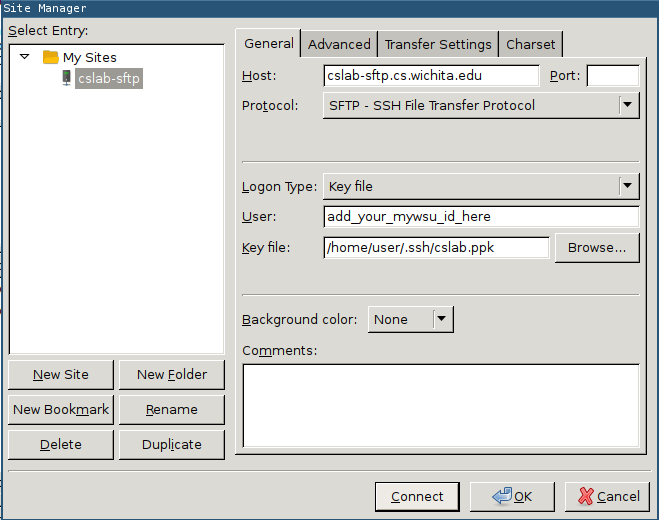
\includegraphics[width=.6\linewidth]{filezilla_cslab_site_manager_linux}
\caption{\textit{FileZilla} Site Manager settings for cslab-sftp}
  \label{fig:pageant}
%% \end{subfigure}%
\end{figure}

%------------------------------------------------
\newpage
\question{Why is \textit{SSH} or \textit{FileZilla} asking to confirm the authenticity of cslab host keys?}\label{host_keys_linux}

\subsection*{Automatically adding the cslab host keys to your known\_hosts file:}
\begin{itemize}
  \item SSH host keys are essential to securing an SSH connection into a remote server. If you see an incorrect host key, then it may mean a cyber-attacker has attempted to compromise the remote server. However, if your configuration loses its cached host keys for any reason, then it may ask you to reconfirm the authenticity of cslab hosts when you try to open an SSH connection.
  \item You can download the \href{https://raw.githubusercontent.com/benroose/tutorials/master/cslab_tutorials/cslab_ssh_client_config_files/cslab_openssh_known_hosts}{cslab\_openssh\_known\_hosts} file and re-add the cslab host keys into you local \verb|known_hosts| file by typing \break
    \verb|cat cslab_openssh_known_hosts >> ~/.ssh/known_hosts|
\end{itemize}

%% \newpage
\subsection*{Manually adding the cslab host keys into \textit{OpenSSH} or \textit{FileZilla}:}
\begin{itemize}
\item If you do not have the cslab host keys in your \verb|known_hosts| file when you initially connect to cslab, you will likely see the following warning:
\begin{verbatim}
The authenticity of host 'cslab.cs.wichita.edu' can't be established.
ECDSA key fingerprint is [SHA256 or MD5 hash value].
Are you sure you want to continue connecting (yes/no)?
\end{verbatim}
\item You can manually add SSH host keys to your \textit{OpenSSH} and \textit{FileZilla} configurations but you should always ensure the host key fingerprint is correct first. \verb|cslab|, \verb|cslab-bastion|, and \verb|cslab-sftp| host key fingerprints must match one of the following SHA256 or MD5 hashes before you add or accept the host key:
\begin{verbatim}
ECDSA key fingerprint is
SHA256:X6dBKj4sqYYPWol6MXSQvGhpIQ6qBxh7mBQhnSw8n64
MD5:d8:ba:c6:1c:86:fa:7f:f6:92:4f:c1:02:30:ce:ab:99

ED25519 key fingerprint is
SHA256:zzozIV7cP1T9C77PLRaevzdzCu21k44lbjd8jaJKS8Q
MD5:6d:3d:8e:3a:db:f6:de:33:af:77:01:40:f3:71:1d:14

RSA key fingerprint is
SHA256:0CUyGZAYMdOd8vTOK3AtM2XTX3lMaGA2NP73rR7s6Ns
MD5:75:5a:16:53:1a:7c:c2:4b:99:66:2d:e3:1e:76:f9:c9

DSA key fingerprint is
SHA256:7zW122xr+aoBb5yiRI96nvdx8Ml07qLKHYwG2Wu6jIM
MD5:27:59:53:18:5a:67:71:f6:32:f1:e1:15:e9:e5:fe:b1
\end{verbatim}

\end{itemize}

%------------------------------------------------

\end{flushleft}
\end{document}
